Sound as we know it can be defined as a physical wave travelling through air or another means. \cite{you_2010} It can be measured as change in air pressure surrounding an object. Once we have this electrical representation of the wave, we can convert it back and consequently play using speakers.

In the real world, these sound waves are generally composed of many different kinds of waves, with differing frequencies and amplitudes. The human ear can tell the difference between high (whistling) and low frequencies (drums), and knowledge of this will be useful later when we are discussing audio encoding.

\begin{figure}[ht]
	\caption[Example audio signal]{An example of an audio signal represented in PCM form.}
	\label{fig:audio_signal}
	\centering
	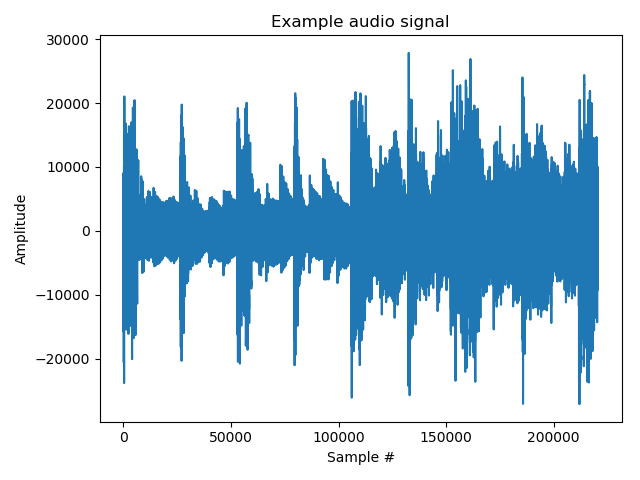
\includegraphics[width=\textwidth]{audio_signal.png}
\end{figure}

\section{Notation}
Below is a summary of the notation this chapter will be using.

\begin{table}[htbp]\caption{Digital audio notation}
\begin{tabular}{r l}
$t$ & symbol representing a time value in seconds \\
$\tau$ & symbol representing a "slow" time, time index with a lower resolution than $t$ \\
$\xi$ & symbol representing a frequency value in hertz \\
$F_s$ & symbol representing a sampling rate of an audio signal \\
$x(t)$ & function representing the amplitude of a continuous signal at a time $t$ \\
$x_n$ & sequence representing the amplitude of a discrete signal indexed by $n$ \\
$w(t)$ & continuous windowing function at a time $t$ \\
$w_n$ & discrete windowing function indexed by $n$ \\
%$X(\xi)$ & function representing the frequency component of a signal for a frequency $\xi$ \\
$S(\xi)$ & the Fourier transform of a continuous signal \\
$S_k$ & the discrete Fourier transform of a discrete signal \\
$S(\tau, \xi)$ & the short-time Fourier transform of a continuous signal \\
$S_{k, \xi}$ & the discrete short-time Fourier transform of a discrete signal \\
$M_k$ & the Modified discrete cosine transform of a discrete signal
\end{tabular}
\end{table}

\section{Important terms}
In this section several terms used throughout this thesis will be described.

\subsection{Sampling}
Sampling in this context refers to the way we convert an analogue signal into a digital one. When we use something like a microphone, what's happening is that it measures the pressure waves generated by the sound around it at regular intervals. The result of this operation is the amplitude of the wave, or the size of the vibration at that point in time.

To obtain an actual usable sound wave of various frequencies and amplitudes, we will need many samples - generally tens of thousands per second. The rate at which we collect these samples is called the \emph{sampling rate}, denoted $F_s$.

\subsection{Nyquist frequency}
It is proven that we can fully represent an arbitrary signal $x(t)$ by its samples $x_n$ \cite{bosi_goldberg_2003}, but there are some conditions to this. If we don't sample a given signal enough times per second, there might be frequencies high enough that our sampler won't be able to record them correctly.

This is called the \emph{Sampling Theorem} and the idea is that we can only accurately record all the frequencies in a signal if our sampling rate $F_s$ is at least twice as large as the largest frequency contained in the signal $F_{max}$. \cite{shannon_sampling_1991}

In essence, a continuous signal can only be fully represented by its samples if:

\begin{align}
F_s \ge 2F_{max}
\end{align}

Looking at it from another angle, it also means that given a sampling rate $F_s$, the highest frequency we can record is equal to $\frac{F_s}{2}$, and that is what's called the \emph{Nyquist frequency} or \emph{Nyquist limit}.

\subsection{Quantization}
Quantization is a process where we restrict a large set of values, possibly continuous, into a smaller set, generally discrete.

For example, when we sample an analogue signal, what we get back is the amplitude represented by a voltage, which can be considered a set of infinitely many real numbers. In order to use these values on our computers for digital processing, these voltages must first be quantized. \cite{bosi_goldberg_2003} An example of a common choice would be signed 16-bit PCM, where each sample is converted to an integer between $-2^{15} = -32768$ and $2^{15}-1 = 32767$, representing the quantized amplitude for the given sample.

Quantization is also common in digital audio processing when we already have discrete values, e.g. when quantizing MDCT values (described later) in order to further reduce the range and allow for more efficient compression.

\subsection{Windowing}
A windowing function $w_n$ is a function that is equal to $0$ outside of some chosen interval, where its value is defined by an expression. It is generally symmetrical, though this is not a rule. Windowing functions are often applied to audio signals by multiplying them with the windowing function before further processing to avoid various artifacts.

There is no one "best window", there's usually a trade off, for example a window used to prevent aliasing will lower the accuracy of frequency identification (as is the case in the Hann window). \cite{bosi_goldberg_2003} In fact, most modern audio codecs use different kinds of windows depending on the musical characteristics of the current block and the ones that follow. \cite{Raissi2002TheTB}

\begin{figure}[ht]
	\caption[Windowing example]{An example of windowing: a sine function windowed by MLT.}
	\centering
	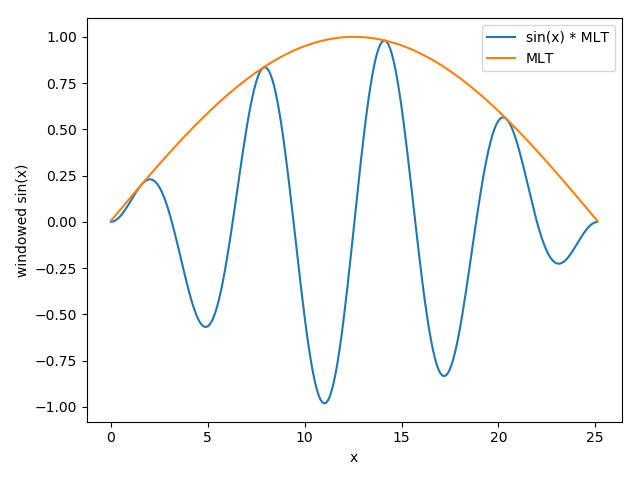
\includegraphics[width=\textwidth]{mlt_window.png}
\end{figure}

\subsubsection{Rectangular window}
The rectangular window is the simplest one, as it does not modify the original signal at all, and as such is often used to represent e.g. a part of a periodic signal. It's equivalent to:

\begin{align}
w_n^R = 1
\end{align}

\subsubsection{Hann window}
A Hann window is a simple sine-based window, defined as:

\begin{align}
w_n^H = \sin^2 \left( \frac{\pi n}{N} \right)
\end{align}

This window is what we'll be using most of the time with the short-time Fourier transform.

\subsubsection{Modulated lapped transform}
Modulated lapped transform (MLT) is another sine-based window, used for example in the MP3 codec. It has a comparatively low computational complexity and is simple to implement. \cite{malvar_1990} It's defined as:

\begin{align}
w_n^M = \sin \left[ \frac{\pi}{2N} \left( n + \frac12 \right) \right]
\end{align}

It is what we will be using with the MDCT due to its simplicity of implementation compared to the results it provides.

\subsubsection{Kaiser-Bessel derived window}
The Kaiser-bessel derived window (KBD) is designed to be used with the modified discrete cosine transform (MDCT), and is used for example in the AC-3 codec. It's defined as follows \cite{bosi_goldberg_2003}:

\begin{align}
w_n^D = \begin{cases}
\sqrt{\frac{\sum_{i=0}^{n}w_i}{\sum_{i=0}^{\frac{N}{2}}w_i}} & \text{if $0 \le n < \frac{N}{2}$} \\
\sqrt{\frac{\sum_{i=0}^{N-1-n}w_i}{\sum_{i=0}^{\frac{N}{2}}w_i}} & \text{if $\frac{N}{2} \le n < N - 1$} \\
0 & \text{otherwise}
\end{cases}
\end{align}

\subsection{Transient}
A transient is a high amplitude sound with a short duration. It's significant because during block-based audio encoding, if a transient occurs on the border between two blocks it may cause what's called \emph{pre-echo} - essentially a type of artifact where a sound is being heard before it should occur.

To mitigate artifacts caused by transients, it's important to use proper windowing.

\subsection{Aliasing}
Aliasing is a type of artifact that occurs when the sampling rate is too low. Due to the way sampling works, frequencies above the \emph{Nyquist limit} are mirrored to lower frequencies, creating a noticeable distortion. \cite{bosi_goldberg_2003}

This can be eliminated by either choosing an appropriately higher sampling rate, or by passing the signal through a low-pass filter to eliminate the higher frequency content that would cause aliasing.

\subsection{Spectral leakage}
As we will see later, the Fourier transform (and other Fourier-related transforms) effectively projects the signal into infinity, as if it was a periodic signal. If we apply the transform to an unmodified signal, it's similar to using a rectangular window on a periodic function, where the signal ends abruptly at the edges. This in turn leads to \emph{spectral leakage} - the resulting Fourier transform will produce non-zero values even for frequencies that aren't contained in the original signal at all.

The way to combat spectral leakage is again, by using proper windowing. By smoothing out the function using a window so that it approaches $0$ along the edges of the signal, we can mitigate some spectral leakage, although not all of it.

\begin{figure}[ht]
	\caption[Spectral leakage example]{An example of a sine function's spectral leakage after application of a rectangular window. Image by \href{https://commons.wikimedia.org/wiki/User:Wdwd}{Walter Dvorak} published under the \href{https://creativecommons.org/licenses/by/3.0/deed.en}{CC BY 3.0} license.}
	\centering
	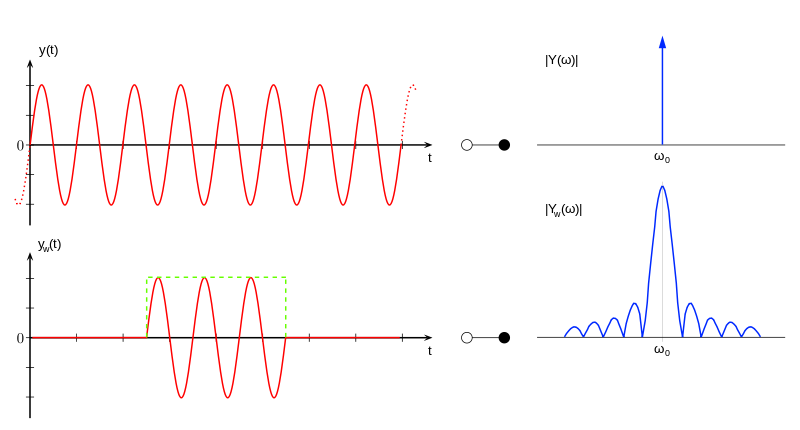
\includegraphics[width=\textwidth]{spectral_leakage.png}
\end{figure}

\subsection{Scalloping}
A phenomena that occurs when using a discrete Fourier (or Fourier-related) transform. Since the frequencies are split into ranges rather than exact values, it's possible that a single frequency may fall into two adjacent bins, providing inaccurate frequency content readings.

To deal with scalloping, a large enough block size in relation to the sampling rate must be chosen to lower the ranges of the bins.

\section{Digital audio representation}
Most commonly, the amount of air pressure is sampled many times a second and after being processed this information is stored as a discrete-time signal using numerical representations - this is what's known as a \emph{digital audio signal}. This entire process is called \emph{digital audio encoding}.

By sampling the audio signal, we will potentially be losing out on some information, but given a high enough sampling rate, the result will be imperceptible to the human ear. For general purpose audio and music, the standard sampling rate is 48 kHz, alternatively 44.1 kHz from the compact disk era.

Once we have our digital signal, there are two distinct kinds of ways we can represent, or, encode it. Both of them have many different data models for encoding \cite{you_2010}, but in this work I am only going to focus on the most relevant ones.

\subsection{Time domain representation}
In the time domain, the signal is simply represented as a function of time, where $t$ is the time and $x(t)$ is the raw amplitude, or air pressure, at that point. \cite{bosi_goldberg_2003}

This is the most straightforward representation since it directly correlates to how the signal is being captured in the first place. However, as we will see later, this format is not ideal for storing audio data with any sort of compression.

\subsubsection{PCM}
In the time domain, the most basic encoding we can use is PCM (Pulse Code Modulation). After sampling a signal at uniform intervals, the discrete values are quantized; that is, each range of values is assigned a symbol in (usually) binary code.

For example using 16-bit signed PCM, each sample will be represented as a 16-bit signed integer, or in the case of multiple channels, N 16-bit signed integers, where N is the amount of channels.

PCM serves as a good base for what we are going to talk about next - Frequency domain representation and encoding.

\subsection{Frequency domain representation}
While it's simple to understand and work with for the computer with samples in the form of a sequence of amplitudes, it's difficult to run any sort of meaningful analysis on such data. To better grasp the structure of the audio we're working with, it would be helpful to be able to decompose it into its basic building blocks, so to speak. And that's where frequency based representation comes in.

The goal here is to represent the signal as not a function of time, but rather a function of frequency $X(\xi)$. That is, instead of having a simple sequence of amplitudes, we will have information about the magnitude for each component from a set of frequency ranges. This description alone is generally more compact than the PCM representation \cite{bosi_goldberg_2003} on top of providing us with useful information about the signal, so it will serve as a good entry point to our compression schemes.

\subsubsection{Fourier transform}
Fourier transform is the first and arguably the most used tool for converting a signal from a function of time $x(t)$ into a function of frequency $X(\xi)$.

It is based on the \emph{Fourier series}, which is essentially a representation of a periodic function as the linear combination of sines and cosines. \cite{Shatkay:1995:FTP:864947} However, the main difference is that our function need not be periodic.

The Fourier transform of a continuous signal $x$ is defined as: \cite{recoskie_mann_2014}

\begin{align}
S(\xi) = \int_{-\infty}^{\infty}x(t)e^{-2\pi it\xi}dt
\end{align}

If we inspect the formula, we can notice that Fourier transform essentially projects our signal into infinity - this wouldn't be a problem if it was a periodic signal, but sampled audio is generally constrained by time. To prevent spectral leakage as a result, we must window the signal before processing it. \cite{heinzel_2002_windows}

The output is a complex number, which provides us with the means to find the magnitude and phase offset for the sinusoid of each frequency $\xi$.

The Fourier transform can also be inverted, providing us with an easy way to obtain the original signal back from its frequency components. The inverse transform is defined as:

\begin{align}
x(t) = \int_{-\infty}^{\infty}S(\xi)e^{2\pi it\xi}d\xi
\end{align}

However, seeing as our samples are discretely sampled, we will need to modify our transform accordingly.

The discrete Fourier transform of a discrete signal $x_0, x_1, ..., x_{N-1}$ is: \cite{Recoskie2014ConstrainedNM}

\begin{align}
S_k = \sum_{n=0}^{N-1}x_ne^{-2\pi ikn/N}
\end{align}

And our inverse is:

\begin{align}
x_n = \frac1N \sum_{k=0}^{N-1}S_ke^{2\pi ikn/N}
\end{align}

In the discrete form, rather than finding the frequency content for a specific frequency $\xi$, we find the content of the $k$-th frequency bin. Since we have fewer values to work with, the frequency range is quantized to a degree and each bin contains an uniformly sized range of frequencies rather than a specific one.

The way that works is as following: if we for example run the discrete Fourier transform on $1152$ samples recorded with a sampling rate $F_s = 44100$, we will end up with $1152$ frequency bins, each containing the amplitude of a frequency range $\frac{F_s}{N} = \frac{44100}{1152} \approx 38$ Hz. However, due to the \emph{Nyquist limit}, the only useful frequencies are up until $\frac{F_s}{2} = \frac{44100}{2} = 22050$ Hz, and so we only need to be concerned with the first half of the bins, i.e. $\frac{1152}{2} = 576$ bins, as the latter half mirrors the first and does not contain any useful information.

Due to the nature of this process, if we run the Fourier transform on our whole signal, we will only be able to analyse it as a whole. That means we won't be able to tell which parts of for example a song are quiet or if there are any parts with very high frequencies - we lose our temporal data.

To alleviate this problem, we can run Fourier transform on smaller chunks of the signal, analyse them separately and later join them back into the original signal. That is the essence of the Short-time Fourier transform.

\subsubsection{Short-time Fourier transform}
When using Short-time Fourier transform, or STFT for short, we first split the signal into smaller segments of equal size and then run Fourier transform on those separately. As such, our output can be projected into two dimensions - specifically a frequency spectrum as a function of time, a spectrogram.

\begin{figure}[ht]
	\caption[Example audio spectrogram]{An example of an audio spectrogram for the signal from Figure \ref{fig:audio_signal}.}
	\centering
	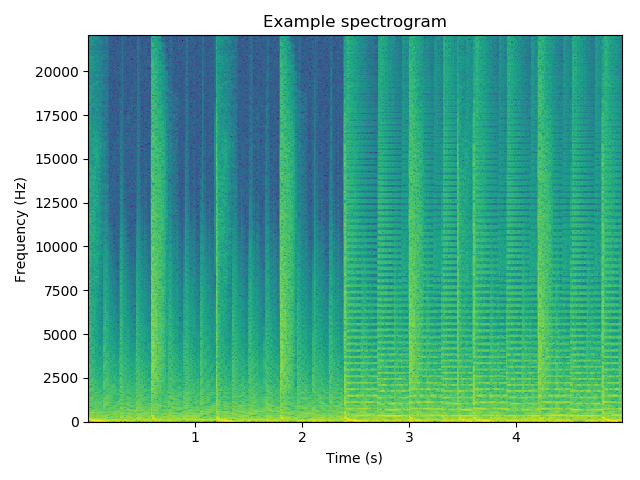
\includegraphics[width=\textwidth]{audio_specgram.png}
\end{figure}

Doing it this way will let us see how the frequency components change over time instead of taking the spectrum of the entire signal.

As with regular Fourier transform, we'll need to window each segment of the signal, but there is a caveat. Since we have windowed segments, we may be losing some information at the edge of each segment leading to artifacts, and furthermore we may be losing information about transients. To solve this, we'll need to introduce overlapping windows - however, having an overlap will increase the amount of coefficients required.

The continuous version is defined as: \cite{Recoskie2014ConstrainedNM}

\begin{align}
S(\tau, \xi) = \int_{-\infty}^{\infty}x(t)w(t-\tau)e^{-2\pi it\xi}dt
\end{align}

where $w$ is the window function.

But again, as we have discrete samples, we will need to use a discrete short-time Fourier transform, specifically:

\begin{align}
S_{k, \xi} = \sum_{n=-\infty}^{\infty}x_nw_{n-k}e^{-2\pi i\xi n}
\end{align}

And similarly to the regular Fourier Transform, short-time Fourier Transform is also invertible. \cite{selesnick_2009}

STFT is commonly used for audio analysis (e.g. for generating spectrograms) but in this case it will be used as a means for our NMF compression.

\subsubsection{Modified discrete cosine transform}
Modified discrete cosine transform, or MDCT for short, has become the dominant means of lossy high-quality audio coding. \cite{wang_vilermo_2012_mdct}

It is what's known as a \emph{lapped transform}. This means that when transforming a block into its MDCT coefficients, the basis function overlaps the block's boundaries. \cite{Malvar:1992:SPL:531523} In practice, what this means is that while we have blocks with overlapping windows as in the short-time Fourier transform, the number of coefficients remains the same as without while retaining the relevant properties.

As the name suggests, MDCT is based on the Discrete cosine transform, namely \emph{DCT-IV}, where the main difference is the addition of lapping mentioned above.

What makes MDCT simpler to work with compared to Fourier transform is that not only do we not need more coefficients despite overlapping, they are also real numbers as opposed to complex numbers, lowering the amount of bytes necessary to store them.

It is a linear function $f: \mathbf{R}^{2N} \rightarrow \mathbf{R}^N$, defined as: \cite{Babu2013FastAE}

\begin{align}
M_k = \sum_{n=0}^{N-1} x_n \cos \left\lbrace \frac{(2n+1+ \frac{N}{2} )(2k+1)\pi }{2N} \right\rbrace
\end{align}

for $k = 0, 1, \ldots, \frac{N}{2}-1$.

It is assumed that $x(n)$ is already windowed by an appropriate windowing function $w$.

MDCT is also invertible, and its inversion is defined as:

\begin{align}
\bar{x}_n &= \sum_{k=0}^{\frac{N}{2}-1} M_k \cos \left\lbrace \frac{(2n+1+ \frac{N}{2} )(2k+1)\pi }{2N} \right\rbrace
\end{align}

for $n = 0, 1, \ldots, N-1$.

It's important to note that the inverted transformed sequence $\bar{x}_n$ by itself does not correspond to the original signal $x_n$ \cite{prince_1986_tdac_1}. To achieve perfect invertibility, we must add subsequent overlapping blocks of the inverted MDCT (IMDCT). This method is called \emph{time domain aliasing cancellation} \cite{prince_1986_tdac_2}, or TDAC for short. As the name suggests, it mainly helps remove artifacts on the boundaries between transform blocks.

\section{Psychoacoustics}
Apart from time-frequency representations being generally more compact, they also give us the ability to analyse, isolate or modify the frequency composition of a given signal. This comprises a large chunk of the audio compressing process.

The field of psychoacoustics studies sound perception - that is, how our ears work and how we perceive different kinds of sounds. There are many different characteristics to sound that need to be taken into account for a proper psychoacoustic analysis \cite{olson1967music}, split into several categories, namely:

\begin{description}
	\item[tonal] includes pitch, timbre, melody harmony
	\item[dynamic] based on loudness
	\item[temporal] involves time, duration, tempo and rhythm
	\item[qualitative] represents harmonic constitution of the tone
\end{description}

For music, it's important to balance these four qualities appropriately. For compression, the most important qualities for us in scope of this work are going to be tonal (pitch) and dynamic (loudness).

\subsection{Pitch}
Pitch is a characteristic that comes from a frequency. The difference between the two is that pitch is our subjective perception of the tone whereas a frequency is an objective measure. Despite this fact, pitch is often quantified as a frequency using Hertz as its unit.

The lower bound of human hearing is around 20 Hz whereas the upper bound is most commonly cited as 20 000 Hz, or 20 kHz. \cite{rosen1993hearing} In a laboratory environment, people have been found to hear as low as 12 Hz. As people age, our hearing gets progressively worse and a healthy adult younger than 40 years can generally perceive frequencies only up to 15 kHz. \cite{olson1967music}

The human ear is capable of distinguishing different frequencies fairly accurately, though accuracy gets lower with increasing frequency. It's easier for our ears to tell a difference between 500 Hz and 520 Hz compared to the difference between 5000 Hz and 5020 Hz. \cite{smacdon_2018}

Furthermore, if we hear two different tones simultaneously, but their frequencies are close enough to one another, we may perceive them as a combination of tones rather than separate tones. Frequency ranges, or bands, where this phenomenon happens, are called \emph{critical bands}. \cite{fletcher_1940} It's also possible for one tone to mask the other entirely, and then we get what's called \emph{auditory masking}. \cite{gelfand1990hearing}

Based on the knowledge of the existence of these critical bands, it's possible to devise a system that specifies the range of each band in human hearing. One such scale that is commonly used is called the \emph{Bark scale}.

\subsubsection{Bark scale}
The Bark scale ranges from 1 to 24 Barks, where each Bark corresponds to a single critical band of human hearing. \cite{fastl_2006} The perceived difference in pitch between each band should be the same, despite the scale not growing linearly in terms of frequency ranges. Specifically, until around 500 Hz, the scale is roughly linear, but above that it has a more logarithmic growth. \cite{hermes_filter}

The Bark scale is commonly used as reference for audio encoding codecs, as we will see later. Knowledge of these critical bands allows for more educated byte allocation during the quantization process when compressing a frequency domain representation.

\begin{figure}[ht]
	\caption[Bark scale]{The Bark scale. Image by \href{https://commons.wikimedia.org/wiki/User:Swpb}{"Swpb"} licensed under \href{https://creativecommons.org/licenses/by-sa/4.0/deed.en}{CC BY-SA 4.0}.}
	\centering
	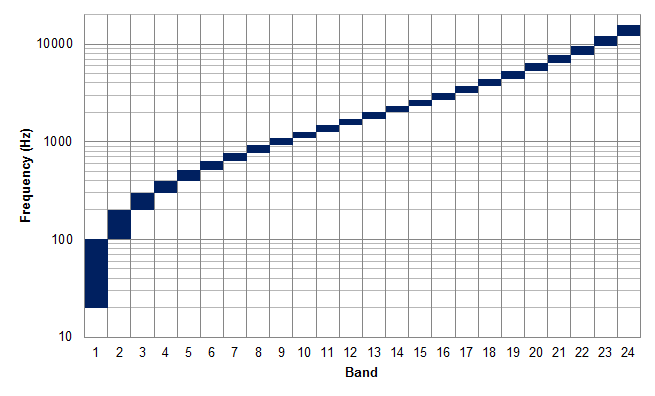
\includegraphics[width=\textwidth]{bark_scale.png}
\end{figure}

\subsection{Loudness}
What people often decide as loudness is really called \emph{sound pressure level} and it's measured in decibels (dB), however it has some shortcomings when it comes to psychoacoustic analysis.

It is defined as following: \cite{behar_1984}

\begin{align}
L_p = 20 \log_{10} \left( \frac{p}{p_0} \right) \text{dB}
\end{align}

where $p$ is a sound's sound pressure and $p_0$ is a reference sound pressure, also called the threshold of human hearing.

While this metric is very popular, it doesn't account for the fact that different frequencies have a different perceived loudness for a person's ears. \cite{olson1967music} There is a lot of research in recent years into how different frequencies impact our perception and hearing \cite{kuwano_1989}, but that is out of scope of this work. For more information about the exact definitions of loudness, refer to \cite{olson1967music}.

\subsection{Auditory masking}
As mentioned above, when it comes to audio masking, and therefore audio compression, we must not only take into account the critical bands as per e.g. the Bark scale, but also their intensity.

For example a lower frequency sound may mask one of a higher frequency, but the other way around does not apply. \cite{gelfand1990hearing} Modern audio encoders take this into account and using this knowledge are able to eliminate sounds that exist in the original signal, but are not perceivable by humans.

There are two important different kinds of masking effects - \emph{simultaneous} masking and \emph{temporal} masking. \cite{Raissi2002TheTB}

Simultaneous masking is what I have hinted at above - when there are two sounds within the same critical band, the dominant one may mask other frequencies within the same band. This can be compensated to a degree by increasing the volume of the masked sound.

Temporal masking does not occur in the frequency domain, but the time domain. The essence is that a stronger tonal component may mask a weaker one if they appear within a small window of time in succession.

\begin{figure}[ht]
	\caption[Auditory masking]{A hypothetical example of how a masker can shift the hearing threshold of a signal by 16 dB. Image created by \href{http://www.highprogrammer.com/alan/}{Alan De Smet} and published in the public domain.}
	\centering
	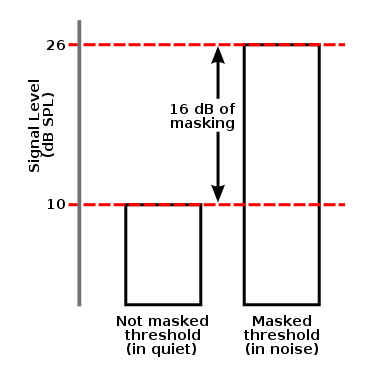
\includegraphics[width=0.7\textwidth]{auditory_masking.png}
\end{figure}
